\chapter{\label{chap:entwurf}Konzeption}
Die erarbeiteten Anforderungen an ein Ampelinformationssystem für FahrradfahrerInnen werden in diesem Kapitel für die Konzeption angewendet. Beginnend mit dem Aufbau der Anwendung werden in den folgenden Abschnitten das Design, die von der Anwendung genutzten Daten, Anwendungsfälle, die Architektur und schließlich die Komponenten der Entwicklumgsumgebung, welche eingesetzt werden aufgeführt. 
\section{Anwendungsaufbau}
Die Anwendungsarchitektur verwendet die Vorgaben für Android-Applikationen. So wird die Hauptkomponente mit Hilfe sogenannter \glspl{Activity} realisiert. Als Basisklasse definiert eine \gls{Activity} das \gls{UI} einer mobilen Anwendung, stellt also die Ansicht mit der BenutzerInnen interagieren können bereit.\\
Eine \gls{Activity} wird von der Bibliotheksklasse \texttt{android.app.Activity} abgeleitet, als Klasse implementiert und muss in der Manifestdatei der \gls{App} aufgeführt werden. \cite{android_activity} \\
In der zu entwickelnden Fahrradapplikation wird keine Navigation innerhalb der Anwendung vonnöten sein, weshalb nur eine \gls{Activity} implementiert wird.
%
% DATENGRUNDLAGE
%
\section{Datengrundlage}
Neben den Daten der eigenen Position ist die Datengrundlage der Ampeln von höchster Priorität. Für die Umsetzung des Prototyps wurde im Rahmen dieser Arbeit als Ausführungsort die Stadt Plau am See in Mecklenburg-Vorpommern festgelegt.\\\\ 
Die Vorteile der Anwendung im ländlichen Bereich liegen in der Verkehrsarmut und die daraus resultierende geringe Menge an Ampeln. Dieser Umstand ermöglicht die Erfassung sämtlicher Ampeln der Stadt, was ein überschaubares Testbild gibt. 
Weiter gibt es keine Straßenbahnen ober Busse, welche den Verkehr durch Grünanforderung beeinflussen. Dadurch lässt sich die Anzahl der Ampeln, bei denen durch Verkehrsabhängigkeit keine Vorhersage möglich ist, minimieren. 

%
% Ampeldaten
%
\clearpage
\subsection{Ampeldaten}
Die Ampeldaten werden manuell erfasst, strukturiert und im \gls{JSON}-Format als Datei auf dem Mobilgerät abgelegt. Um einen Überblick zu gewähren, werden die wichtigsten Komponenten skizziert. \\\\
\begin{minipage}{0.6\textwidth}
Jede Kreuzung hat unterschiedliche Schaltpläne, die zu festgelegten Tageszeitabschnitten greifen. Die Tabelle \ref{tab:zeitplan} zeigt, wie ein solcher Tagesplan einer Kreuzung aussehen kann, wobei an anderen Tagen die Uhrzeiten sowie die Reihenfolge, Quantität und Dauer der Zeitschaltprogramme variieren können.\\\\
Für jedes Schaltzeitprogramm existiert ein Signalschaltzeitplan der Informationen über die Ampelbezeichnung der Kreuzung und deren Rot-, Grün, Gelb, Rotgelb und Dunkelphasen. In letzterer ist die \gls{LSA} ausgeschaltet, was zum Beispiel nachts häufiger der Fall ist. 
\end{minipage} \hspace{1cm}
\begin{minipage}{0.3\textwidth}
	\begin{tabular}{@{}cc@{}}
	\toprule
	\rowcolor[HTML]{ECF4FF} 
	\multicolumn{2}{l}{\cellcolor[HTML]{ECF4FF}\textsc{\centering \large Bezeichnung der Kreuzung}}   \\ \midrule
	\rowcolor[HTML]{EFEFEF} 
	\multicolumn{1}{l}{\cellcolor[HTML]{EFEFEF}\textbf{Uhrzeit}} & \multicolumn{1}{l}{\cellcolor[HTML]{EFEFEF}\textbf{Schaltprogramm}} \\ \midrule
05:00 & Früh   \\ \midrule
11:00 & Tag    \\ \midrule
17:00 & Spät   \\ \midrule
23:00 & Nacht  \\ \bottomrule

\end{tabular}
\captionof{table}{Zeitschaltplan}	 
\label{tab:zeitplan}
\end{minipage}
\\ \vspace{0.5cm} \\
Die Abbildung \ref{fig:plan} zeigt auf, wie so ein Schaltzeitplan für eine Kreuzung mit vier Ampeln aussehen kann. Der Buchstabe R in der Bezeichnung steht hierbei für "'Radfahrampel"'. \\
\begin{figure}[H]
\centering
	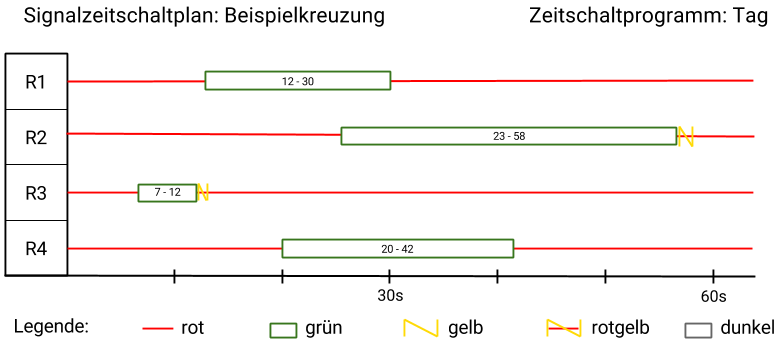
\includegraphics[width=0.8\textwidth]{szplGoogle}
	\rule{36em}{0.5pt}
	\caption[Signalplan]{Beispielhafter Signalschaltplan einer Kreuzung}
	\label{fig:plan}	
\end{figure}
In dem oben gezeigtem Beispiel steht demnach die Ampel R1 zwischen 11 und 17 Uhr in jeder Minute für die Sekunden 12 - 30 Grün und den Rest der Zeit Rot.\\\\
%\begin{figure}[H]  
%    \centering  
%    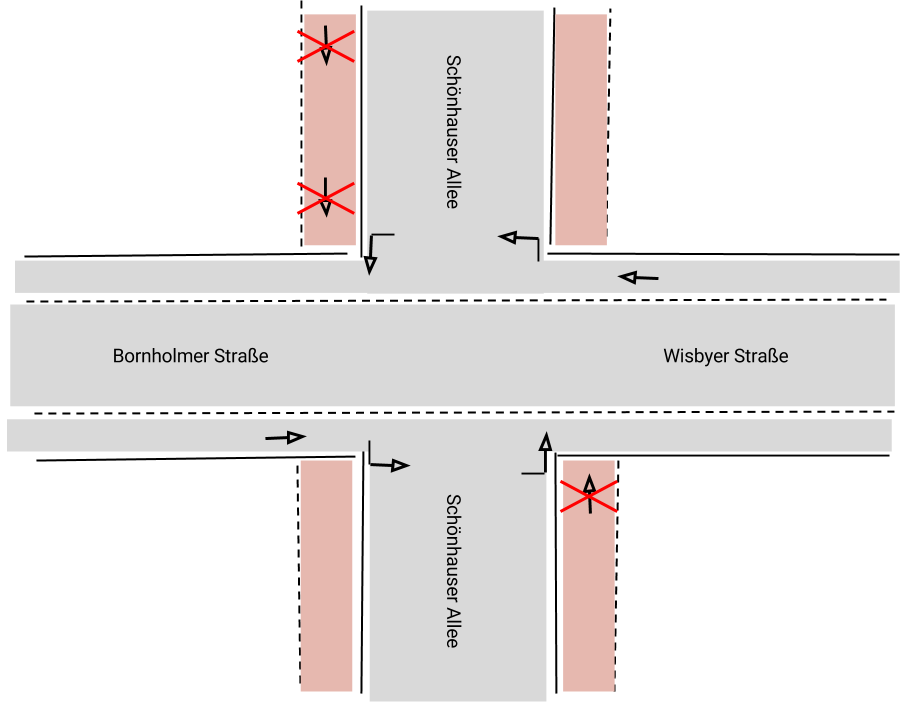
\includegraphics[width=0.7\textwidth]{kreuzung} 
%    \rule{35em}{0.5pt}
%    \caption{Lageplan}
%    \label{fig:kreuzung}
%\end{figure}
Auch die Position jeder Ampeln wird händisch erfasst und in das WGS84-Format konvertiert, um dann zusammen mit den Phasendaten in das gewählte \gls{JSON}-Format gebracht zu werden.\\
Als Referenzzeit ist die Zeit zwischen 12 und 16 Uhr von Freitag bis Montag gewählt. Diese kann selbstverständlich bei Bedarf ausgedehnt bis vervollständigt werden.
%
% LSA als JSON
%
\subsection[Ampelobjekt im JSON-Format]{Ampelobjekt im \gls{JSON}-Format}
\gls{JSON} ist ein leichtgewichtiges, auf JavaScript basierendes, Datenaustauschformat, das für Menschen gut les- und schreibbar und für Maschinen einfach analysier- und generierbar ist. Ein \gls{JSON}-Objekt besteht aus einer von zwei Grundstrukturen. Eine Auflistung von Schlüssel/Wert Paaren oder eine geordnete Liste von Werten, als Array realisiert. Der folgende Codeabschnitt zeigt beispielhaft ein \gls{JSON}-Ampelobjekt:  
\begin{center}
\rule{35em}{0.5pt}
\lstinputlisting[language=JSON, caption=JSON-Ampelobjekt]{code/lsas.json}
\rule{35em}{0.5pt}
\end{center}
Das hier aufgeführte Ampelobjekt hat den Namen \texttt{SteinstraßeA1}, welcher auf die Kreuzung auf der sich die Ampel befindet schließen lässt. Es folgen die zwei Werte \texttt{lat} und \texttt{lon}, die die genaue Position der \gls{LSA} beschreiben und der boolsche Wert \texttt{dependsOnTraffic}, der auf \texttt{false} gesetzt ist, sobald die Ampel verkehrsunabhängig ist. Im anderen Fall ist sie verkehrsabhängig und fällt somit aus den Berechnungen heraus, benötigt also auch keine weiteren Daten. Das Array \texttt{timetable} beinhaltet Schaltplanobjekte mit einem Array aus Tagen und der Start-und Endzeiten an denen diese gelten. Die Werte \texttt{greenFrom} und \texttt{greenTo} bezeichnen den Start und das Ende jeder Grünphase des Schaltplans. Da als Referenzzeit die Zeit zwischen 12 und 16 Uhr gewählt wurde, werden die Schaltpläne welche diese nicht betreffen nicht aufgenommen.
%\subsection{Fahrraddaten}
%Position und Geschwindigkeit werden mittels \gls{GPS} ermittelt.
%erst nach Änderung der Position Aktion...?
% ### USE CASES ###
\clearpage
\section{Anwendungsfälle}
Aus den in Kapitel \ref{chap:anforderungen} beschriebenen Anforderungen und den in Kapitel \ref{chap:szenarien} erarbeiteten Szenarien ergeben sich die folgenden fünf Use-Cases, die von der Anwendung erfüllt werden sollen.\\
\begin{table}[H]
\centering
	\begin{tabular}{@{}>{\columncolor[HTML]{ECF4FF}}l ll@{} p{0.1\textwidth}p{0.4\textwidth}p{0.4\textwidth}} \toprule	
\multicolumn{1}{c}{\cellcolor[HTML]{ECF4FF}\textbf{ID}} 
& \multicolumn{1}{c}{\cellcolor[HTML]{ECF4FF}\textbf{Anwendungsfall}} 
& \multicolumn{1}{c}{\cellcolor[HTML]{ECF4FF}\textbf{Beschreibung}} \\ \hline
% UC1
\multicolumn{1}{l}{\cellcolor[HTML]{ECF4FF}\textbf{UC2}} & \multicolumn{1}{p{0.35\textwidth}}{Ich fahre langsamer, um die grüne Ampel zu passieren}
& \multicolumn{1}{p{0.55\textwidth}}{Der Countdown der aktuellen Ampelphasendauer wird sekündlich aktualisiert und zusätzlich zur Aufforderung langsamer zu fahren angezeigt} \\ \midrule
% UC2
\multicolumn{1}{l}{\cellcolor[HTML]{ECF4FF}\textbf{UC1}} & \multicolumn{1}{p{0.35\textwidth}}{Ich fahre schneller, um die grüne Ampel zu passieren}
& \multicolumn{1}{p{0.55\textwidth}}{Es wird eine Beschleunigungsaufforderung ausgesprochen. Unterstützend wird der Countdown der aktuellen Ampelphasendauer sekündlich aktualisiert und zusätzlich angezeigt} \\ \midrule
% UC3
\multicolumn{1}{l}{\cellcolor[HTML]{ECF4FF}\textbf{UC3}} & \multicolumn{1}{p{0.35\textwidth}}{Ich halte meine Geschwindigkeit, um die grüne Ampel zu passieren}
& \multicolumn{1}{p{0.55\textwidth}}{Die aktuelle Geschwindigkeit ist genauso hoch wie die berechnete Empfehlungsgeschwindigkeit. Es wird angezeigt, dass kein Handlungsbedarf besteht, also das Tempo gehalten werden kann.}\\ \midrule
% UC4
\multicolumn{1}{l}{\cellcolor[HTML]{ECF4FF}\textbf{UC4}} & \multicolumn{1}{p{0.35\textwidth}}{Ich muss in jedem Fall bei roter Ampel anhalten}
& \multicolumn{1}{p{0.55\textwidth}}{Die berechnete Empfehlungsgeschwindigkeit übersteigt die festgelegte Höchstgeschwindigkeit oder die zu erreichende Beschleunigung ist in dem Maße nicht zu erreichen, also ist die Distanz zur Ampel zu lang. Eine Anzeige mit dem Signal "'keine Weiterfahrt ist möglich"' erscheint.}\\ \midrule
%UC5
\multicolumn{1}{l}{\cellcolor[HTML]{ECF4FF}\textbf{UC5}} & \multicolumn{1}{p{0.35\textwidth}}{Es ist nicht möglich eine Vorhersage zu treffen}
& \multicolumn{1}{p{0.55\textwidth}}{Eine verkehsrabhängige Ampel mit individueller Steuerung nähert sich. Es ist dem System nicht möglich eine wahrscheinliche Vorhersage zu treffen und so die entsprechende Empfehlung auszusprechen. Es wird \textit{ein gelbes Fragezeichen, symbolisch dafür} angezeigt.}\\ \bottomrule \cellcolor[HTML]{FFFFFF} \vspace{0.1cm}
\end{tabular}
\rule{35em}{0.5pt}
	\caption{Anwendungsfälle}	
	\label{tab:uc}
\end{table}
Das in Abbildung \ref{fig:uc} gezeigte Use-Case-Diagramm veranschaulicht die in der obigen Tabelle \ref{tab:uc} aufgeführten Anwendungsfälle.  
\begin{figure}[H]  
    \centering  
    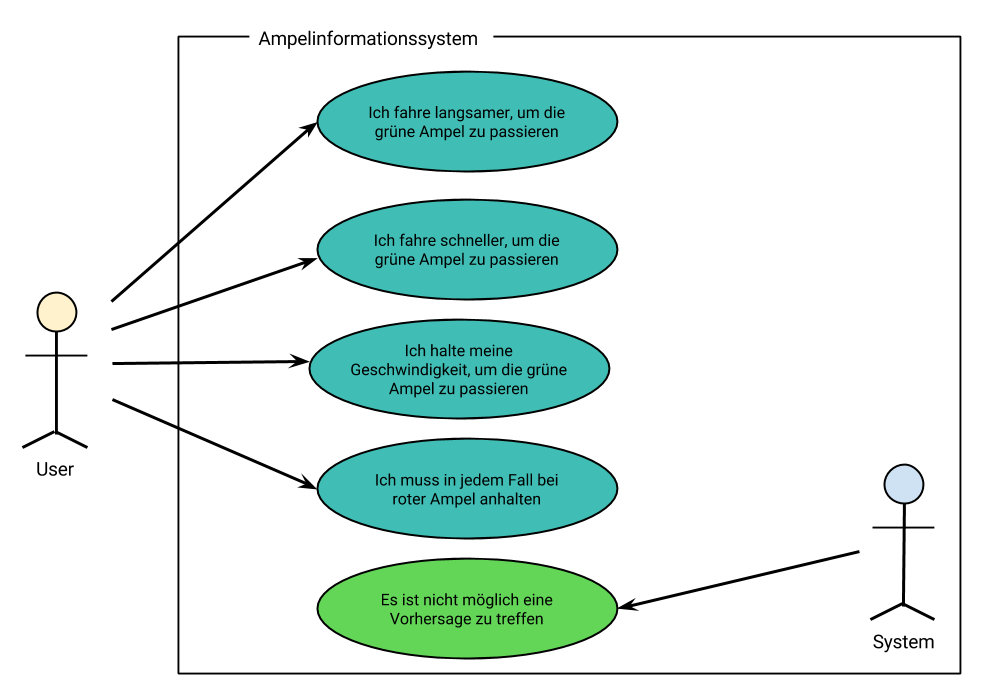
\includegraphics[width=0.8\textwidth]{uc} 
    \rule{35em}{0.5pt}
    \caption{Use-Case-Diagramm}      
    \label{fig:uc}
\end{figure}
\section{Klassenarchitektur}
Die zu erstellende Anwendung erhält den Namen AIS, was für Ampel-Informationssystem steht und der vorläufige Name der Anwendung ist und besteht aus den nachfolgend beschriebenen Klassen. \\\\
Die \texttt{MainActivity} ist die Hauptklasse der Android-Applikation. Sie definiert die grafische Oberfläche der Anwendung und stellt die notwendigen Methoden bereit. \\
Der \texttt{\gls{JSON}Parser} liest die erstellte \gls{JSON}-Datei ein und wandelt deren Inhalt ein ein Array um. Dieses Beinhaltet Ampelobjekte mit deren Namen, Position und der Information darüber, ob sie verkehrsabhängig sind oder nicht. Sind sie es nicht, wird außerdem zu jeder Ampel ein Array, bestehend aus den Sigalschaltplanobjekten gespeichert. Diese enthalten benötigten alle Informationen über den Geltungszeitraum und der Grünphasen.\\ 
\texttt{GPSTracker} implementiert die Schnittstelle \texttt{LocationListener} und kann so kontinuierlich die Position des Endgeräts verfolgen. Mit der eigenen Position und der aller Ampeln aus dem vom \texttt{JSONParser} erstellten Array ermittelt er außerdem die nächste Ampel. Ist diese identifiziert, wird über den \texttt{OnSetListener} die Klasse \texttt{SpeedHandler} aktiviert, welche anhand der Daten aus dem Signalschaltplanobjekt den Countdown der Rotanzeige und die optimale Geschwindigkeit berechnet und die Anzeige entsprechend aktualisiert. \\
Das nachfolgende Klassendiagramm gibt eine Übersicht über die oben beschriebenen Klassen.
\begin{figure}[H]  
    \centering  
    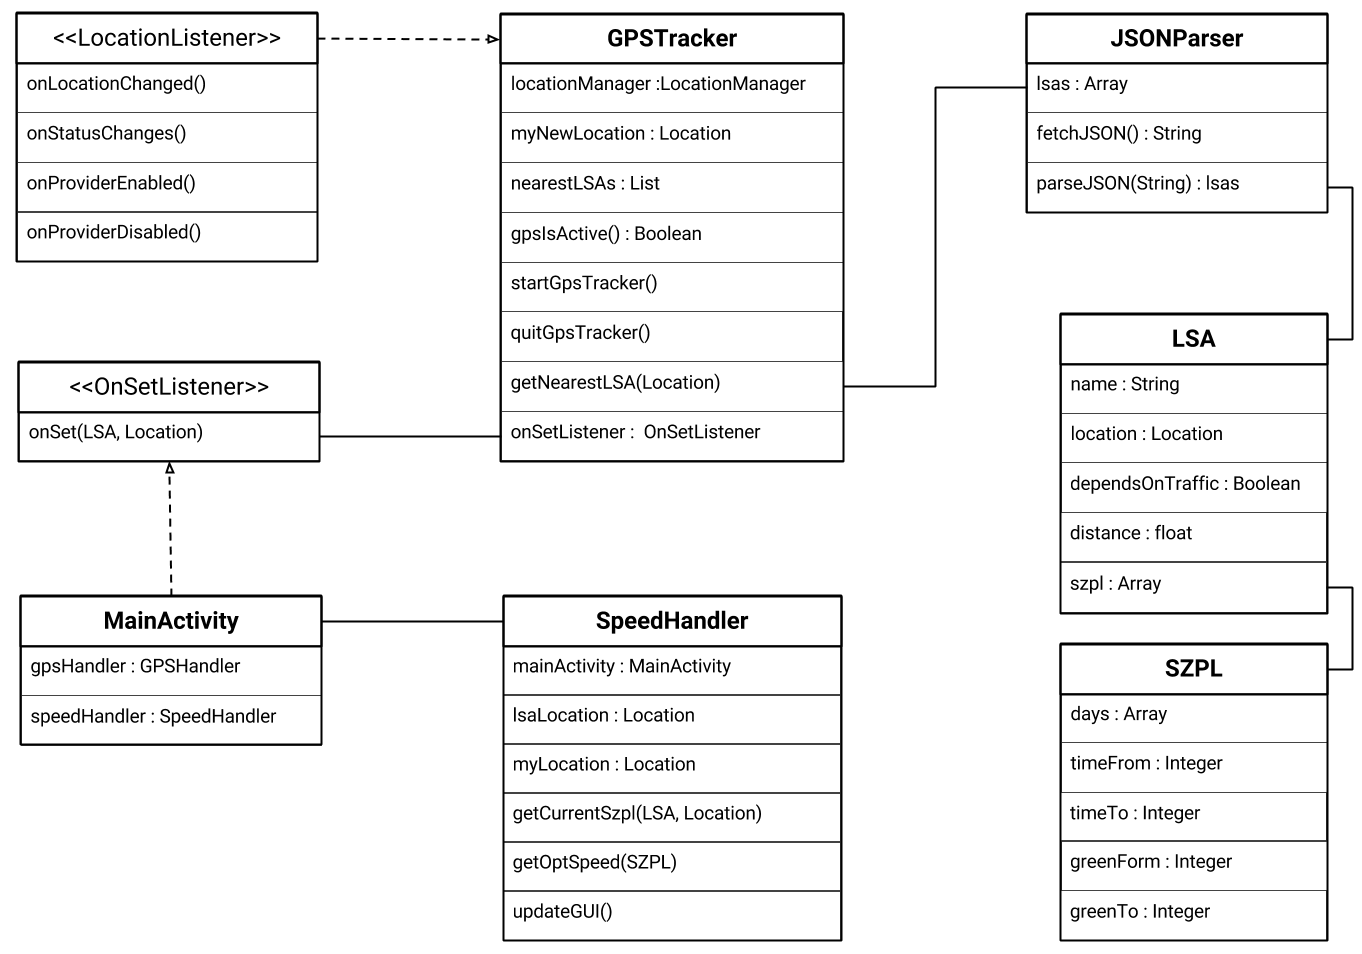
\includegraphics[width=\textwidth]{uml} 
    \rule{35em}{0.5pt}
    \caption{Klassendiagramm}
    \label{fig:uml}
\end{figure}
% ### Design ###
%\clearpage
\section{Die graphische Oberfläche}
Aus den Anforderungen an die graphische Oberfläche in Kapitel \ref{chap:anforderungen} entsteht das Design. Durch die überschaubare Anzahl an Funktionalitäten kann der Aufbau einfach gehalten werden. Aus den Empfehlungsanzeigen, welche den Systemzuständen entsprechen sind vier Ansichten abzuleiten. Die folgende Abbildung zeigt den Entwurf der Benutzeroberfläche.
Abbildung \ref{fig:stop} zeigt die grapfische Umsetzung des Zustands \textit{a}, in dem die Ampelschaltung keine Weiterfahrt ermöglicht. Es wird ein großer roter Kreis mit einem schwarzen Kreuz verwendet. Rot ist eine Signalfarbe und steht auch bei Ampeln für "'Halt"' oder "'Stop"'. Auch das Kreuz wird häufig als \textit{verweigerndes} Symbol eingesetzt und ist somit intuitiv als solches erkennbar.\\
Abbildung \ref{fig:yeah} setzt die Visualisierung des Zustands \textit{b} um, bei dem man mit der aktuellen Geschwindigkeit in der Grünen Welle fährt, um. Hier wird ist ein großer grüner Kreis verwendet, in der Mitte steht "'ok"'. Durch die nicht alleinige Benutzung der Ampelfarben Rot und Grün ist die Ansicht auch für Menschen mit einer Rot-Grün-Sehschwäche eindeutig interpretierbar.
\begin{figure}[H]
        \centering
           \begin{subfigure}[t]{0.18\textwidth}
                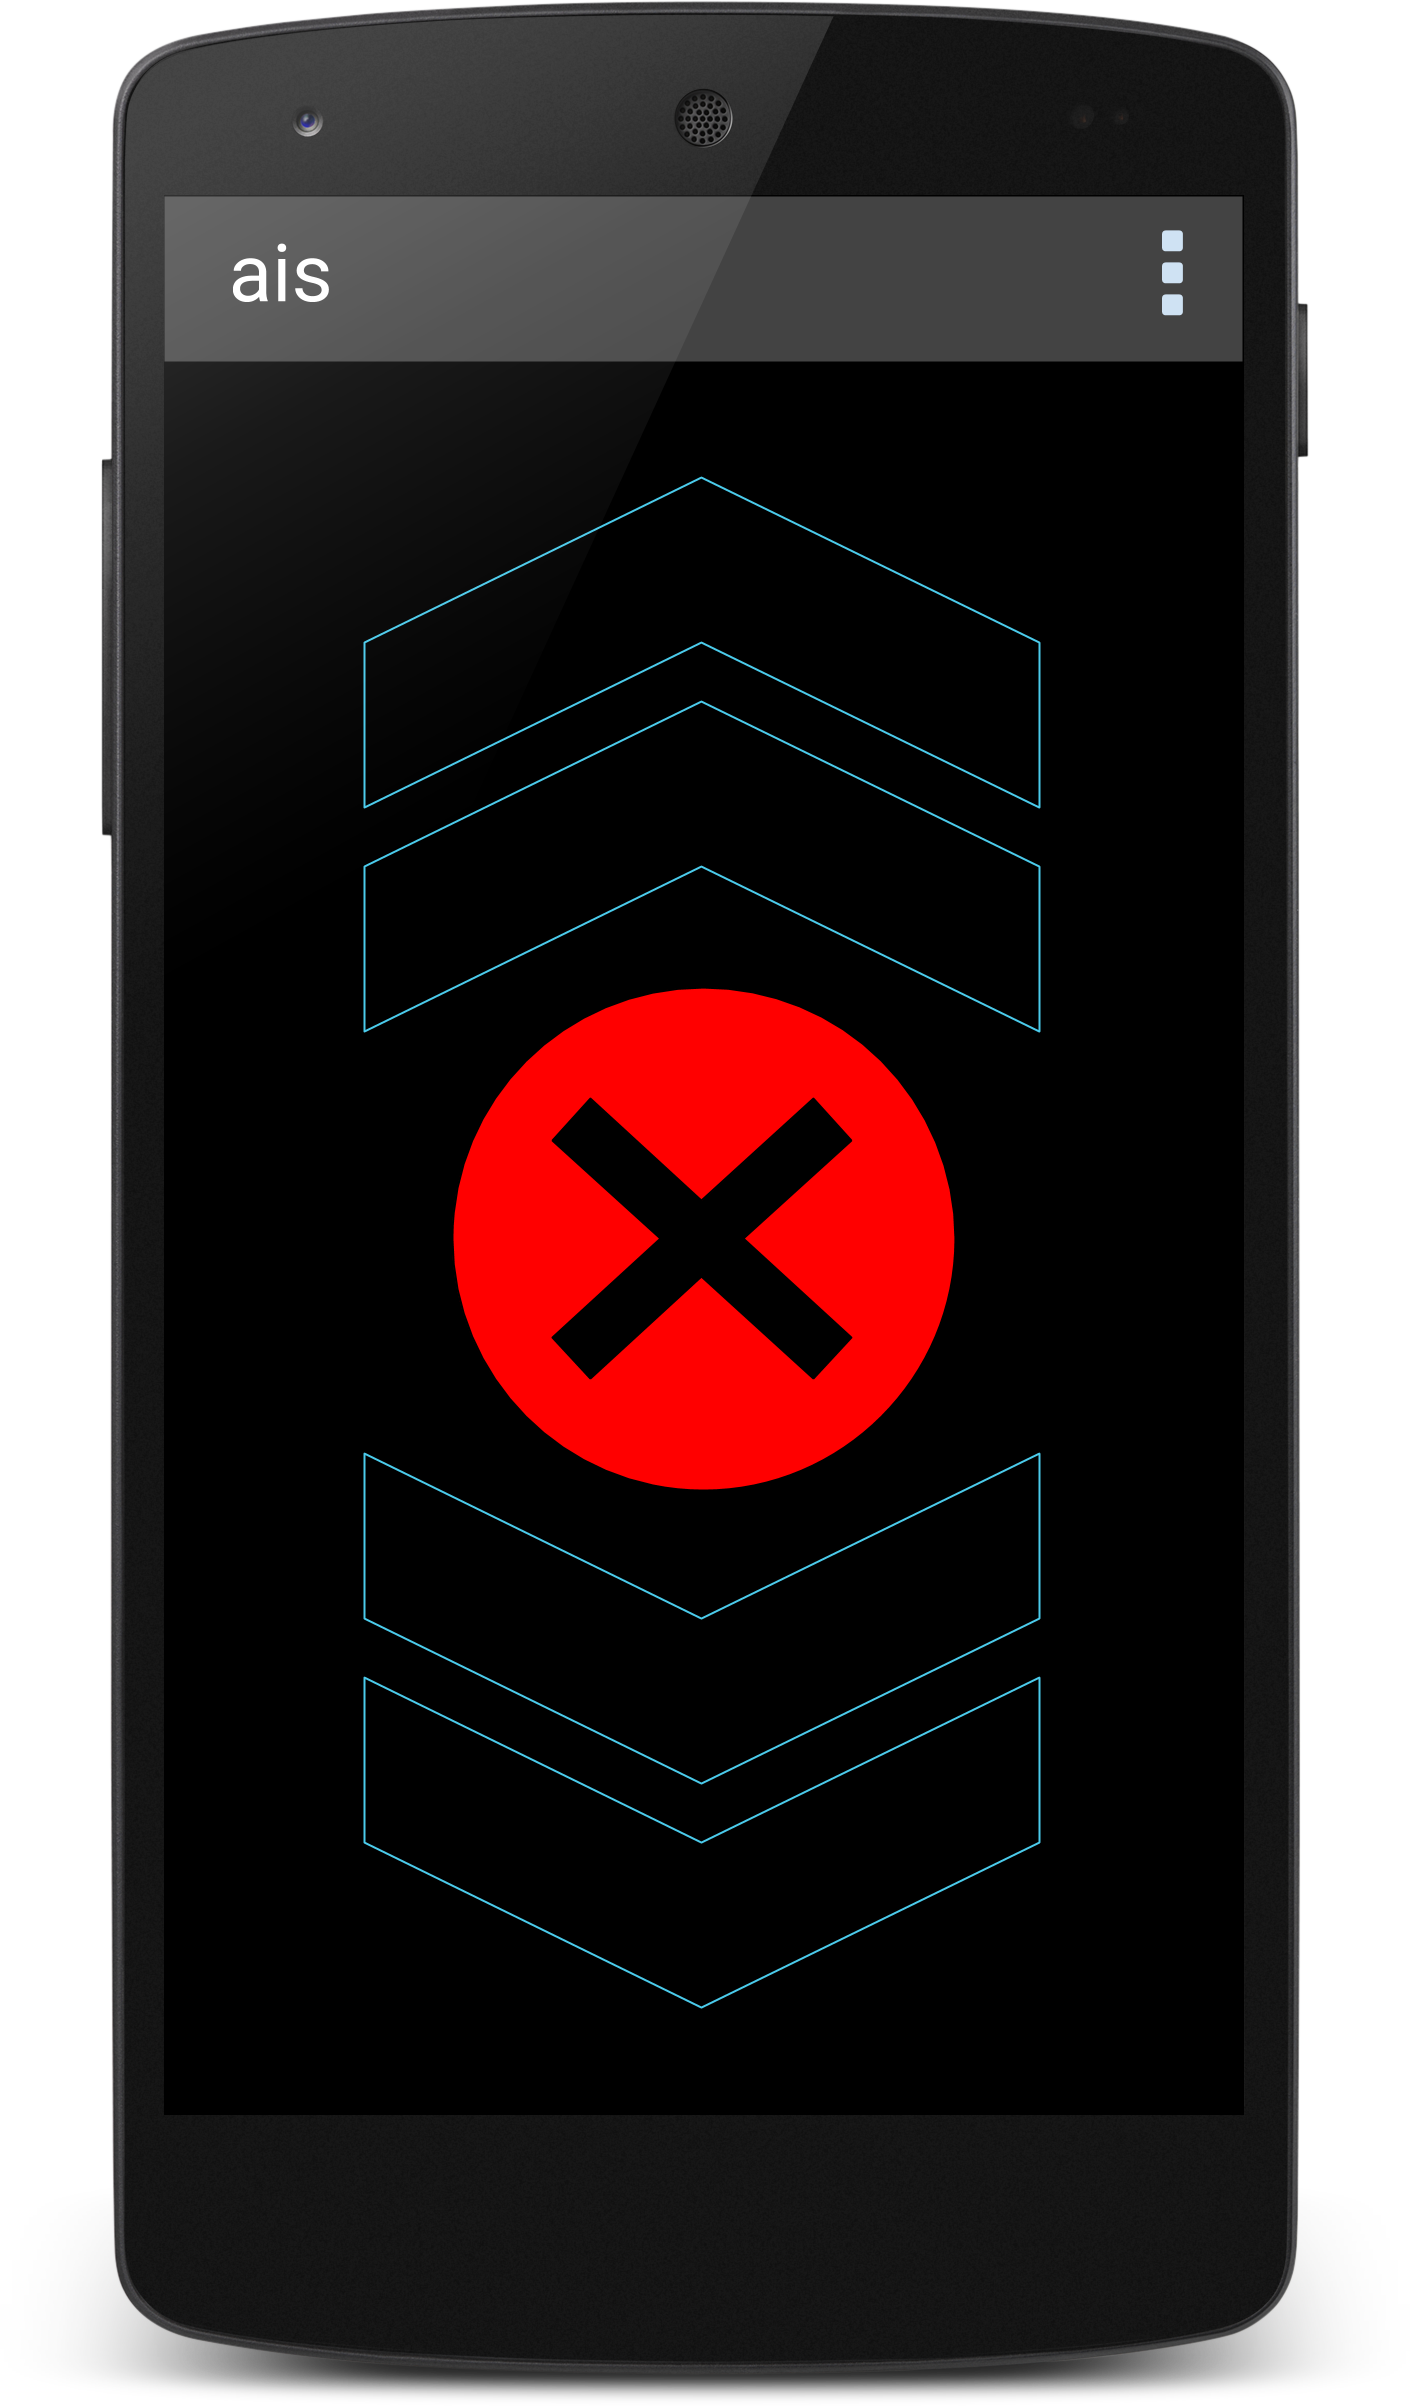
\includegraphics[width=\textwidth]{stop}
                \caption[Systemzustand a]{Anhalten an roter Ampel in jedem Fall erforderlich}
                \label{fig:stop}
        \end{subfigure}
           ~ 
              \begin{subfigure}[t]{0.18\textwidth}
                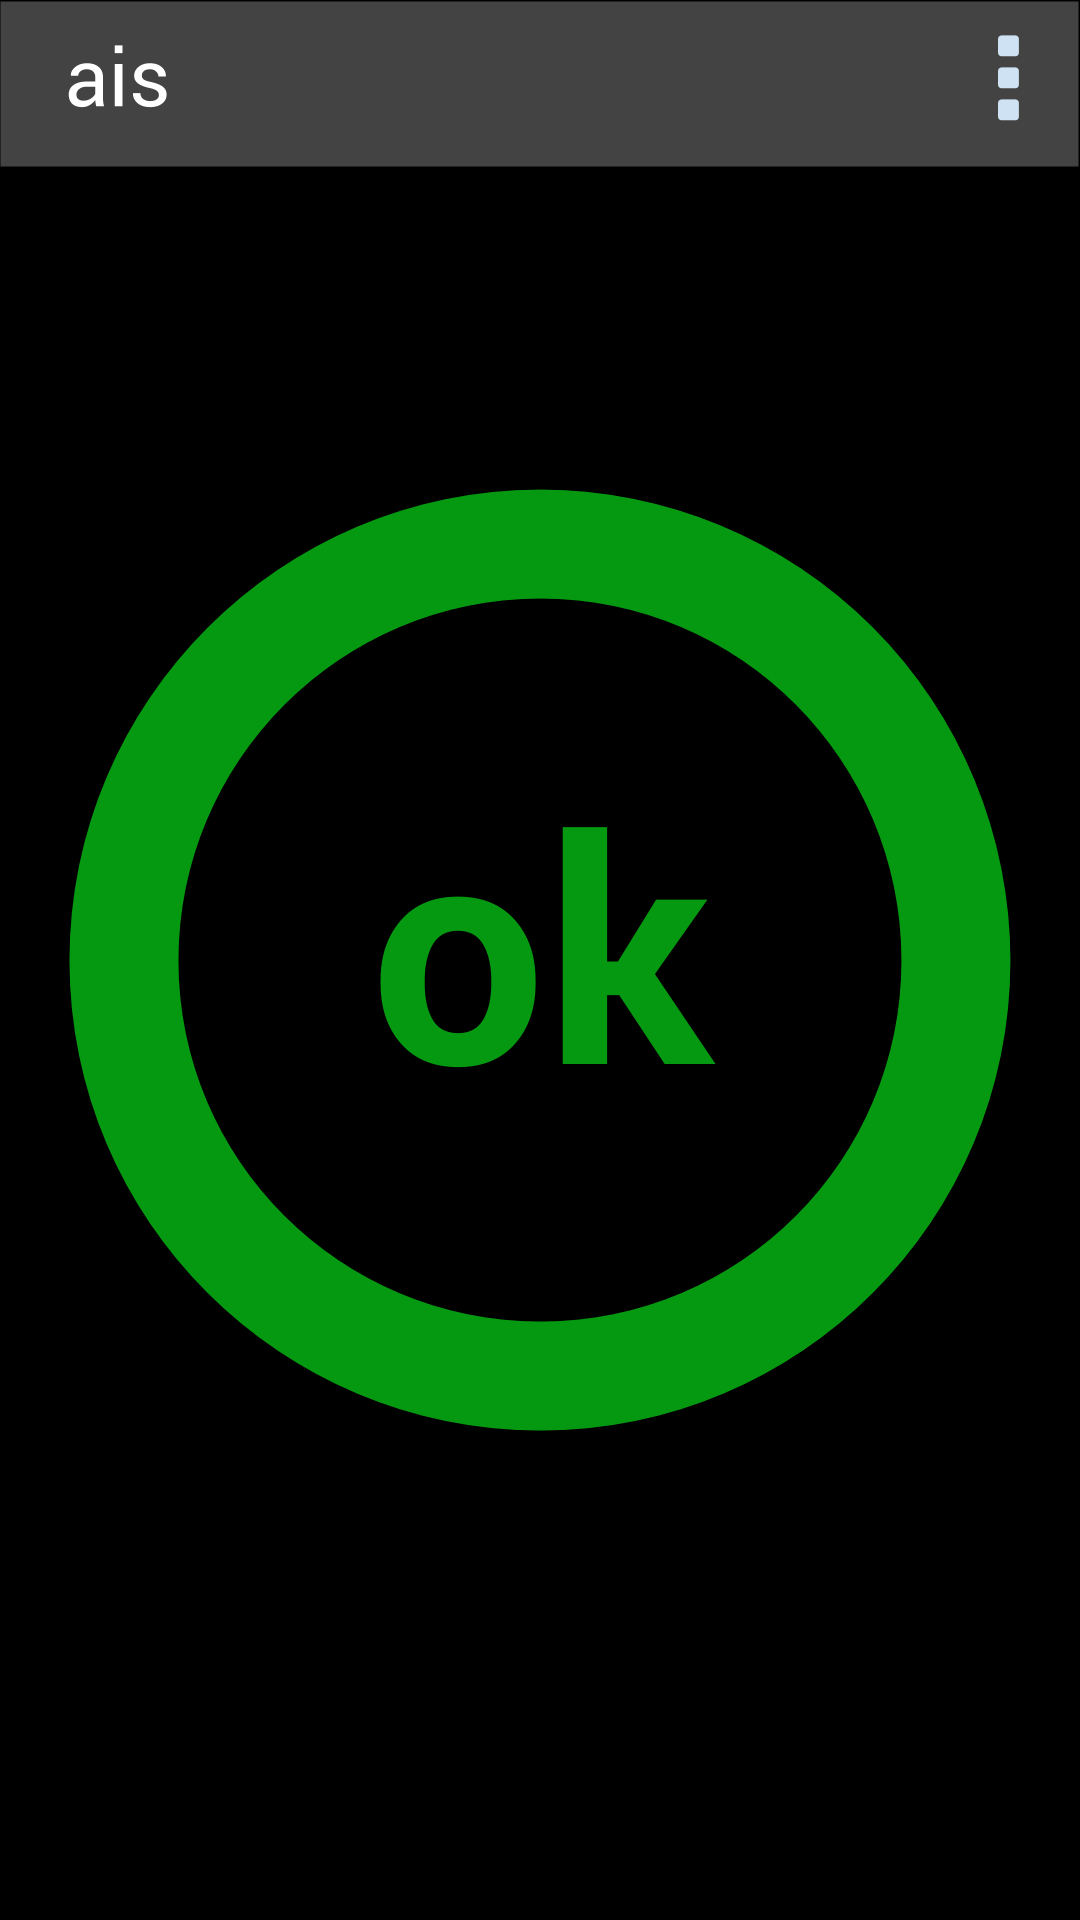
\includegraphics[width=\textwidth]{yeah}
                \caption[Systemzustand b]{Kein Aktionsbedarf}
                \label{fig:yeah}
        \end{subfigure}
           ~
        \begin{subfigure}[t]{0.18\textwidth}
                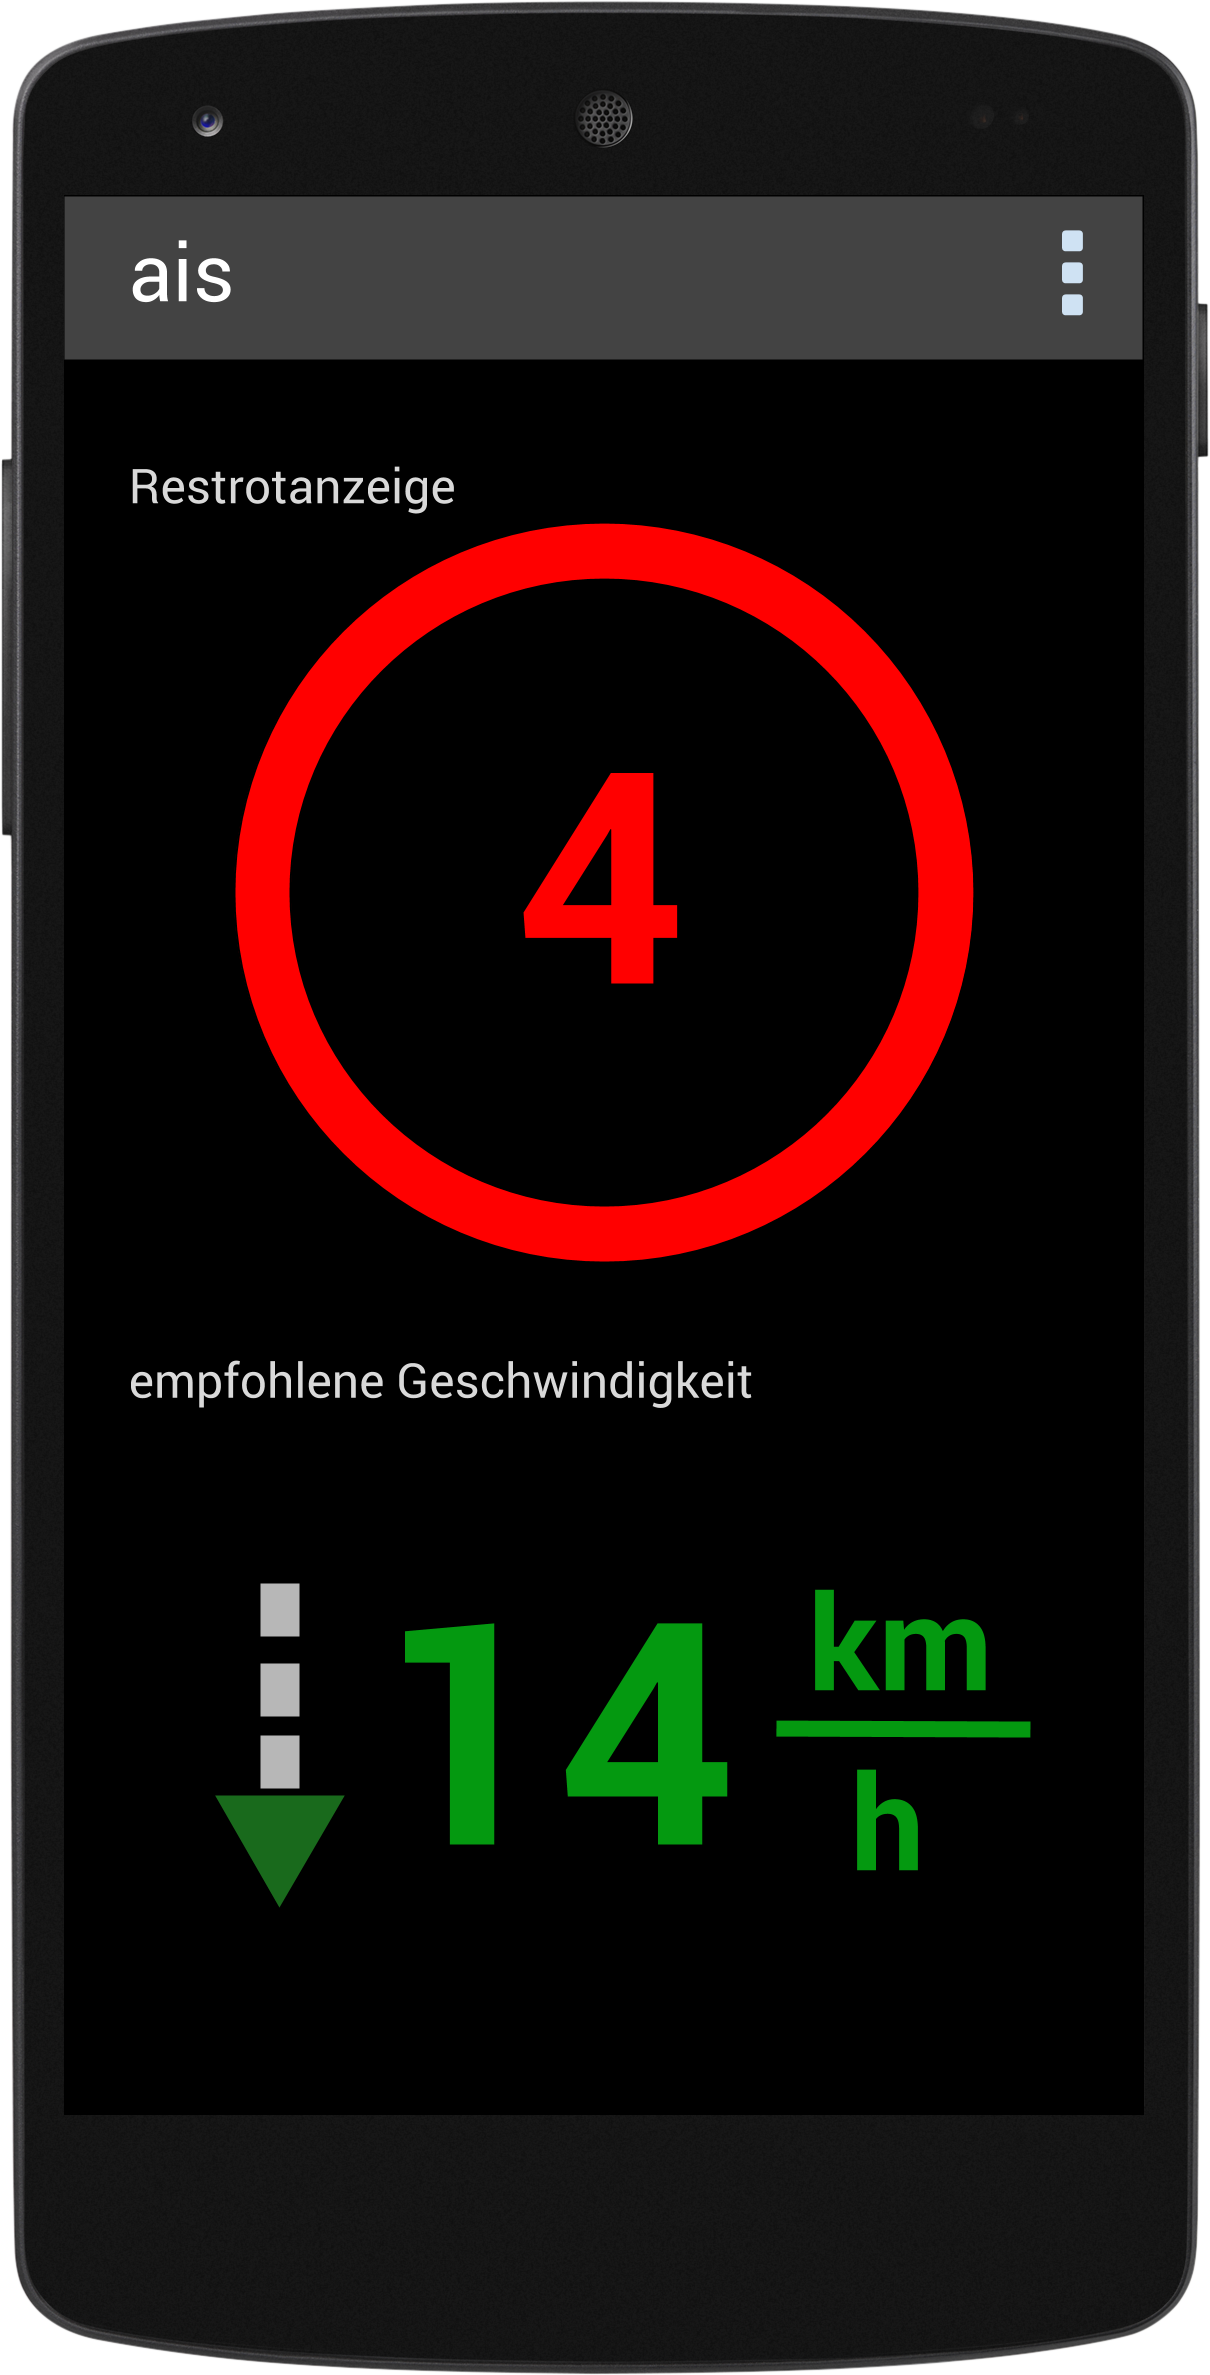
\includegraphics[width=\textwidth]{langsamer}
                \caption[Systemzustand c]{Weiterfahrt durch Verlangsamung  möglich}
                \label{fig:langsamer}
        \end{subfigure}
        ~
        \begin{subfigure}[t]{0.18\textwidth}
                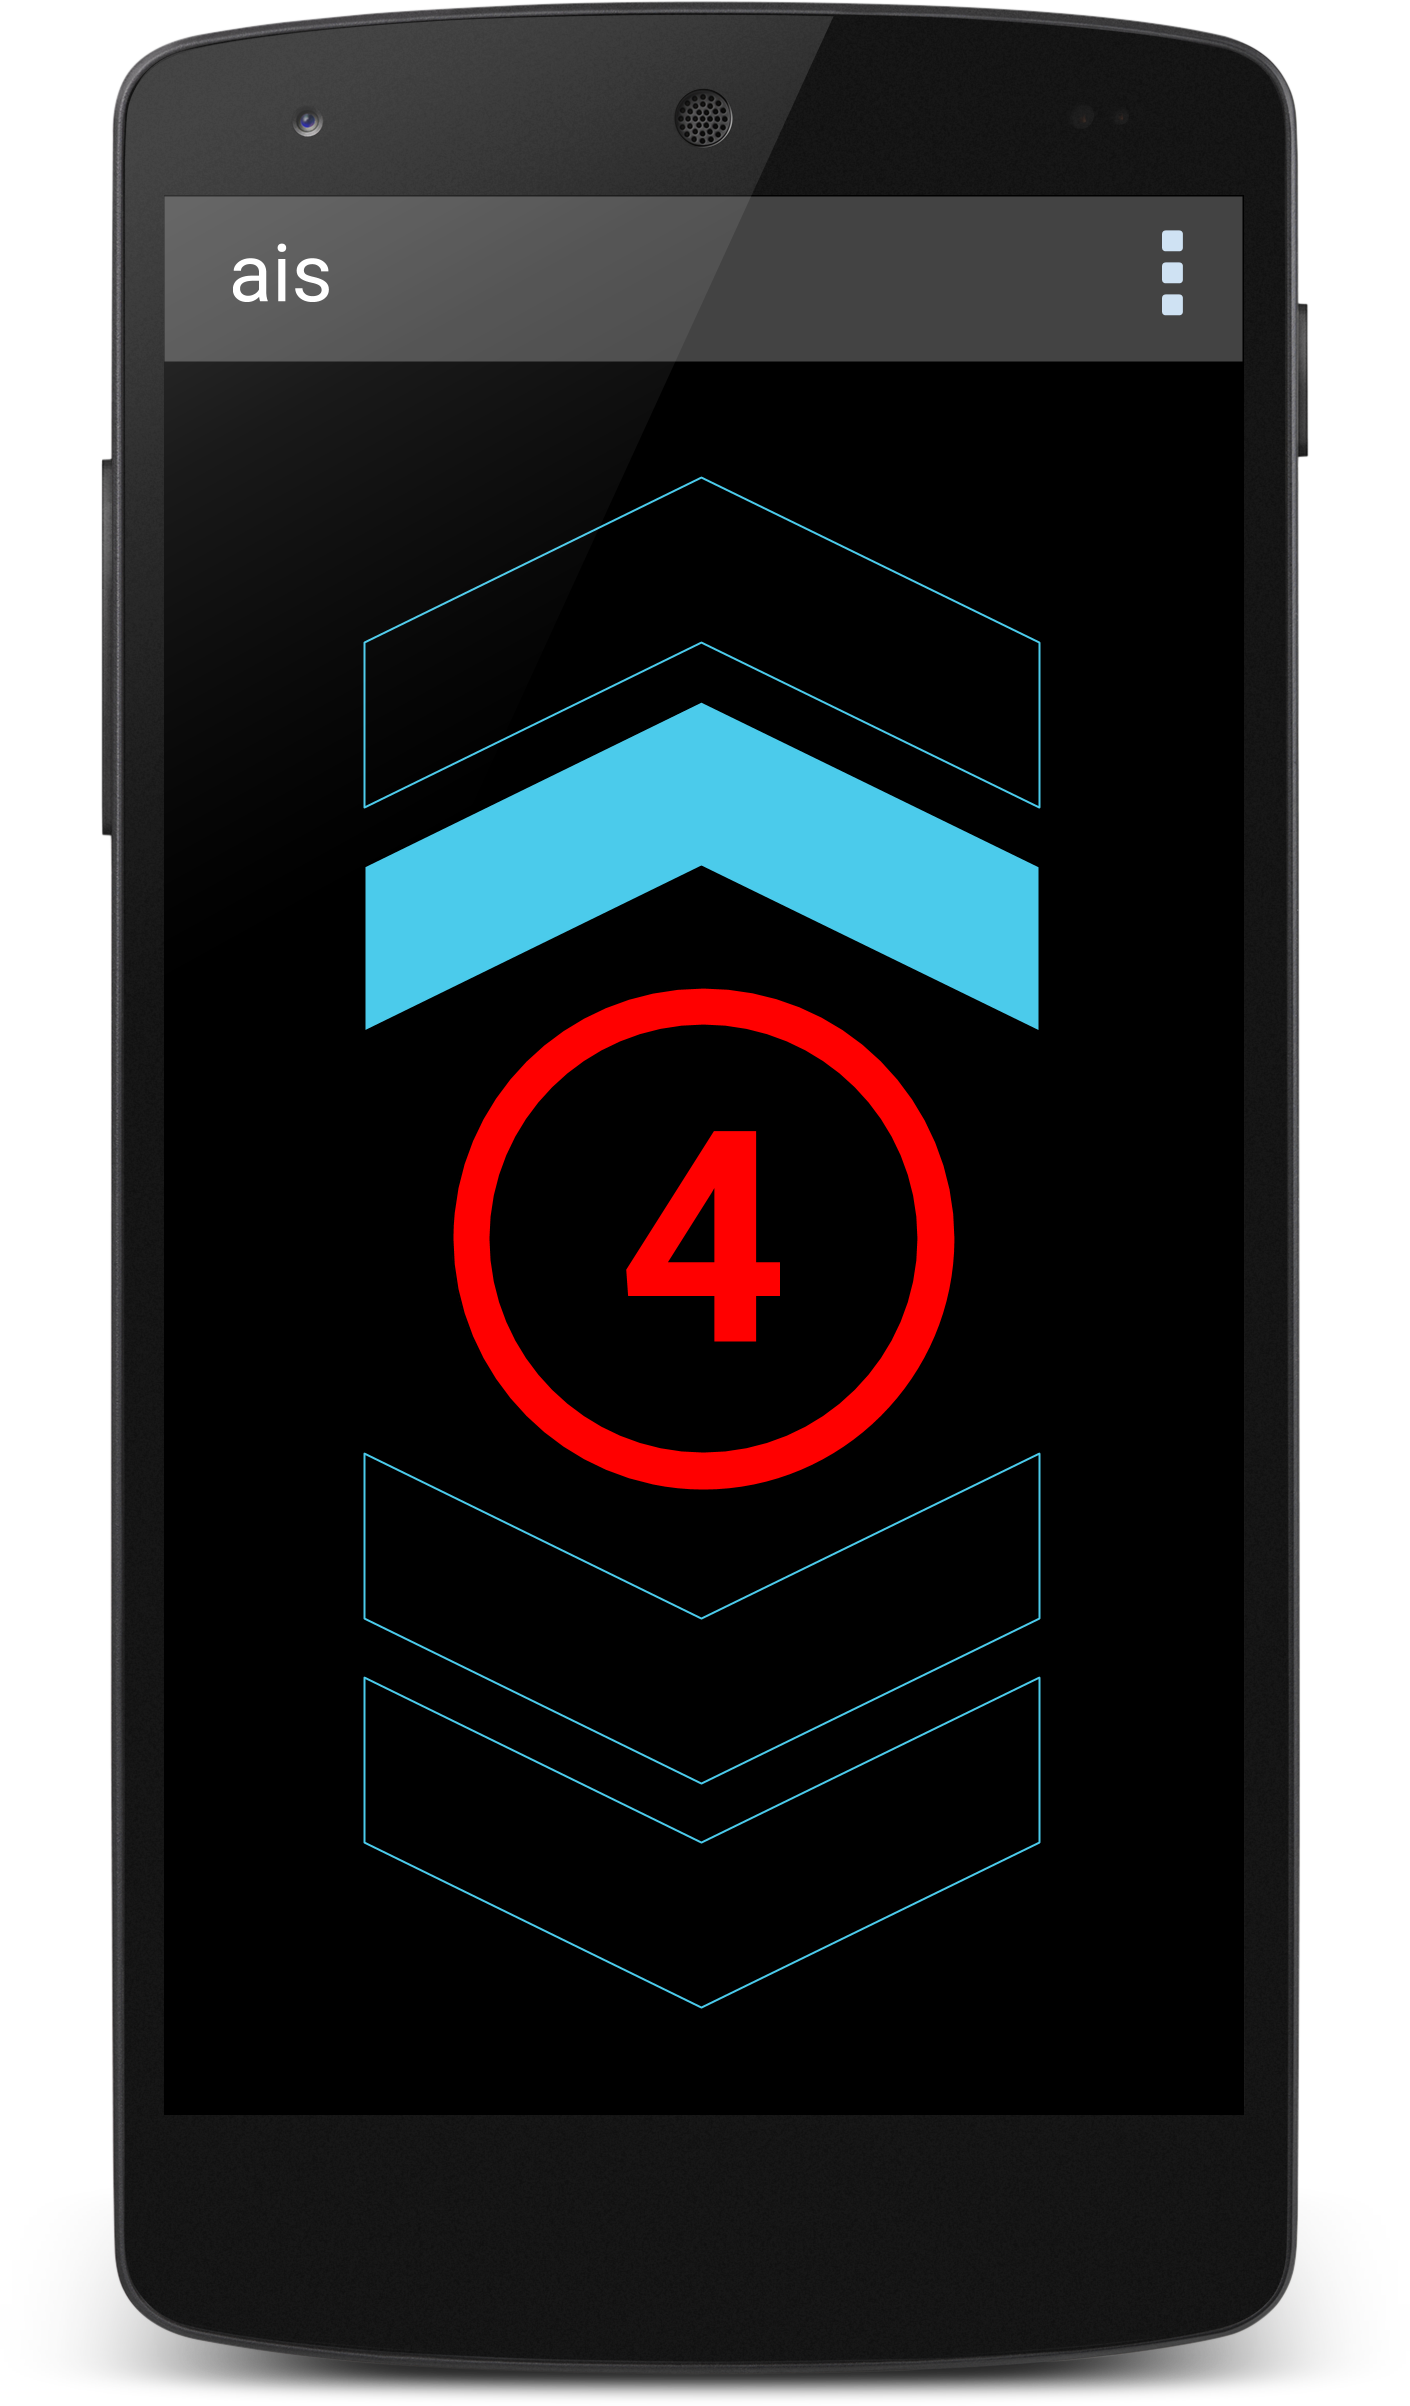
\includegraphics[width=\textwidth]{schneller}
                \caption[Systemzustand d]{Weiterfahrt durch Beschleunigung möglich}
                \label{fig:schneller}
        \end{subfigure} 
        ~ 
        \begin{subfigure}[t]{0.18\textwidth}
        	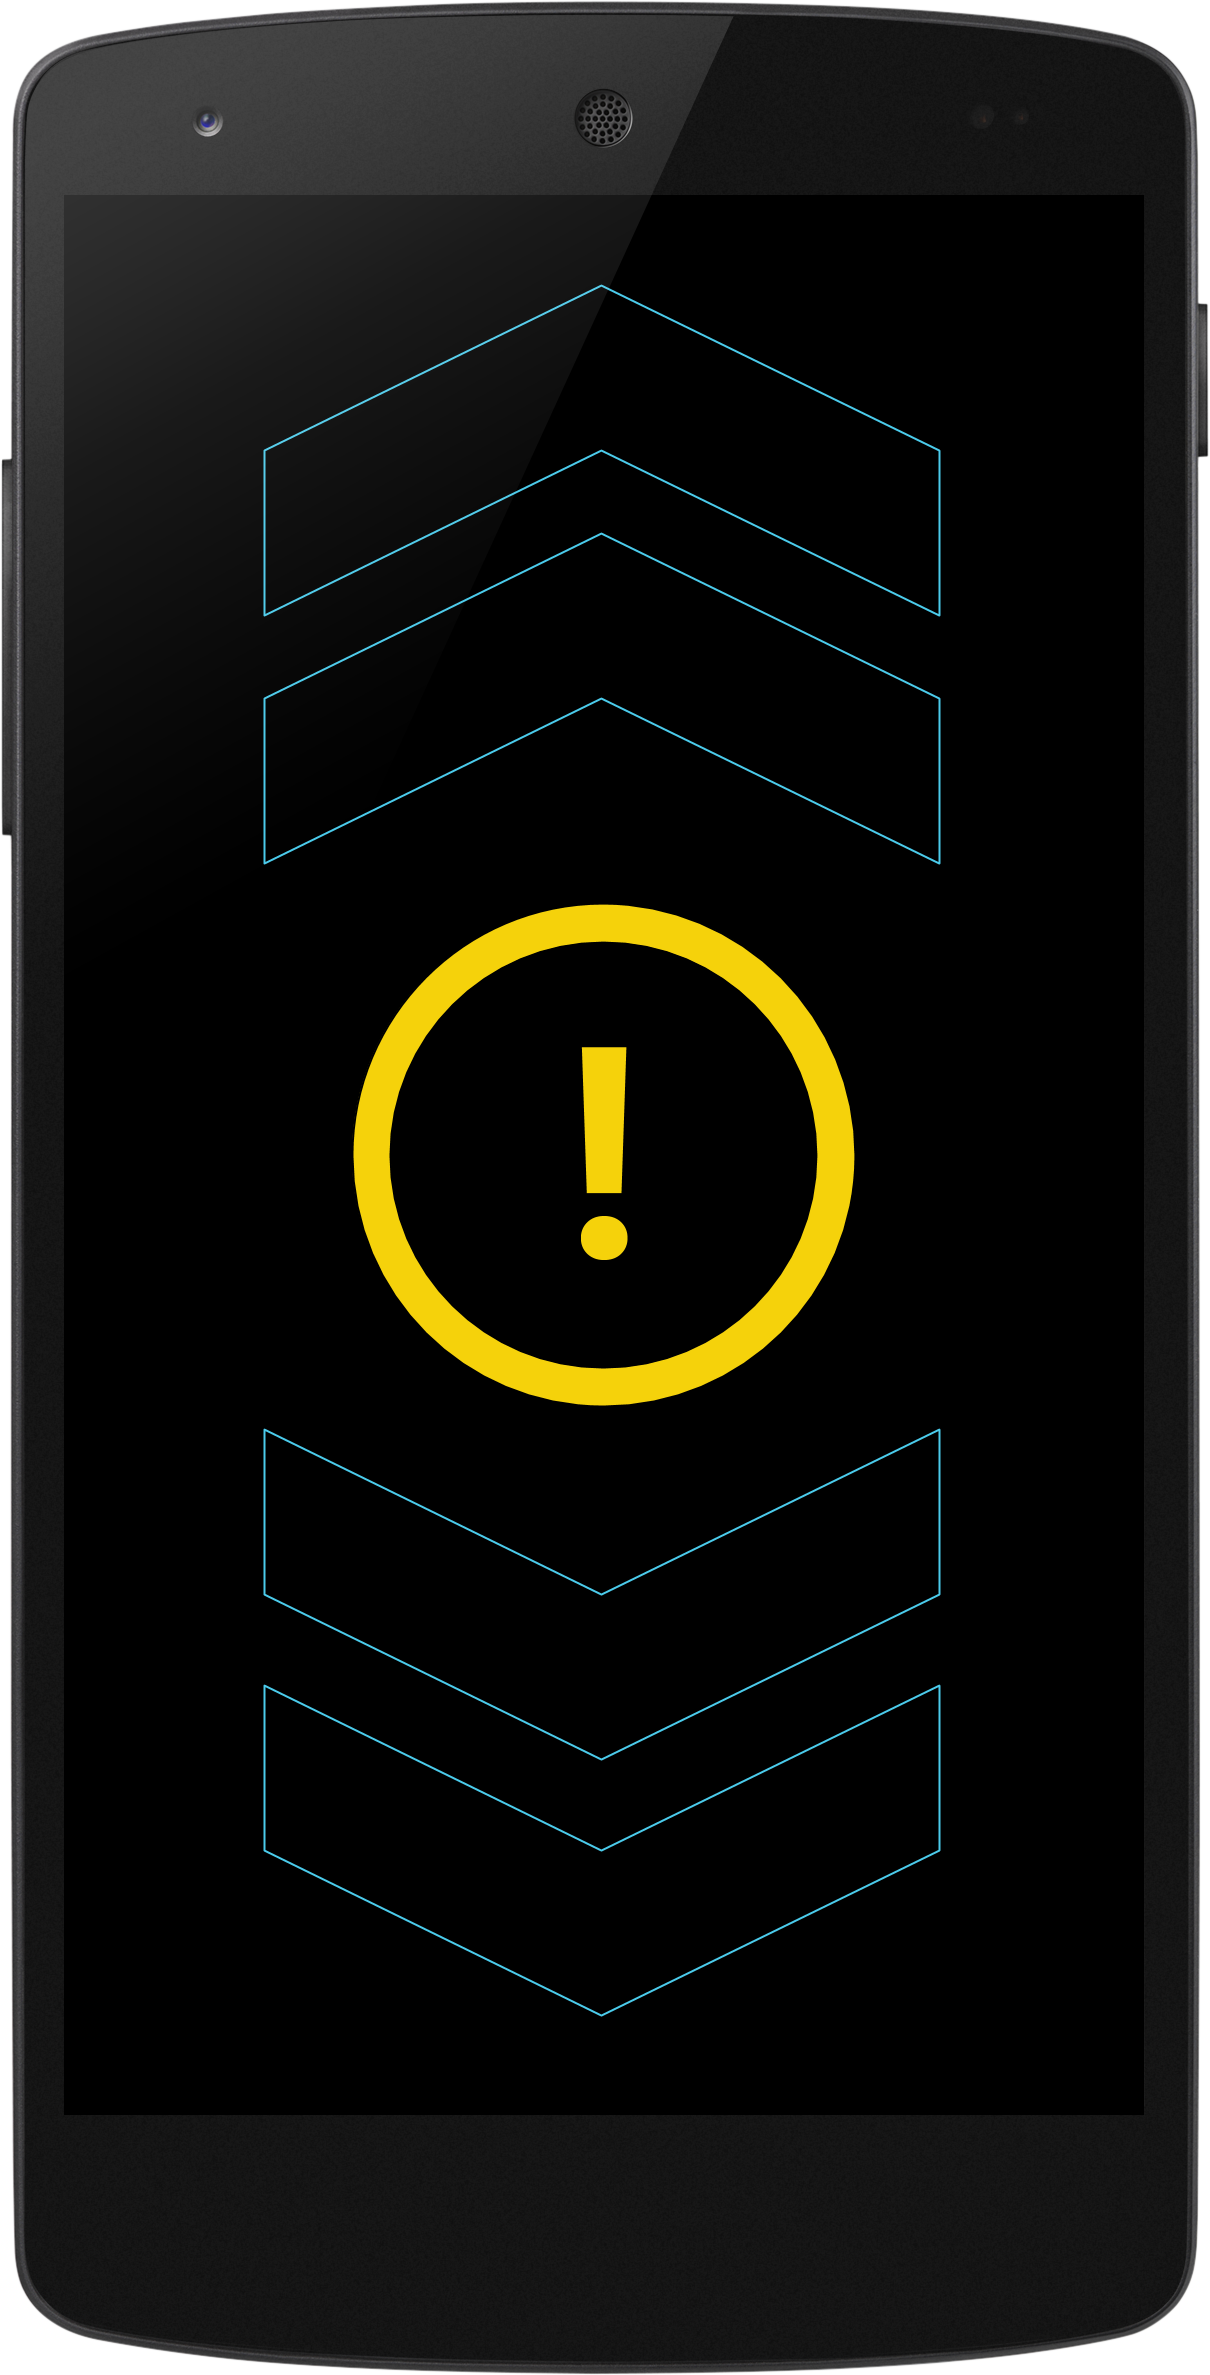
\includegraphics[width=\textwidth]{mep}
        	\caption[Systemzustand e]{Keine Vorhersage möglich}
            \label{fig:meh}
        \end{subfigure} 
        \rule{35em}{0.5pt}   
        \caption[Systemzustände im Ampelbereich]{Entwurf des Designs anhand der Systemzustände}
        \label{fig:mockup}
\end{figure}
Die Abbildungen \ref{fig:langsamer} und \ref{fig:schneller} für die Zustände \textit{c} und \textit{d} sind in der Anordnung der Elemente identisch. Mittig im Bild ist eine eingekreiste rote Zahl die den Countdown der Restrotanzeige darstellt. Sie wird also mit jeder Sekunde aktualisiert. Ober- und unterhalb des Countdowns befinden sich jeweils zwei hellblaue Pfeile. Je nach Differenz der aktuellen zur berechneten Geschwindigkeit sind ein oder zwei Pfeile ausgefüllt. Wird also empfohlen viel schneller zu fahren, sind die oberen Pfeile aktiv, bei der Aufforderung etwas das Tempo zu drosseln der untere. Es sind immer alle Pfeile zu sehen. Durch die Anzeige "'ein von zwei"' ist die Bedeutung der Geschwindigkeitsstufen klarer. Als Farbe für die Pfeile wurde Hellblau gewählt. Sie unterscheidet sich sowohl farblich als auch in der Helligkeitsstufe zu den anderen Farben und steht im hohen Kontrast zu dem Hintergrund. Auf schwarzem Hintergrund wirken die Farben intensiver und sind so auch aus dem Augenwinkel leichter zu erkennen und unterscheiden. Die in Abbildung \ref{fig:meh} gezeigte Darstellung erscheint, wenn keine Vorhersage möglich ist weil die Ampel verkehrsabhängig und die Vorhersage dadurch zu ungenau wird. Als Farbe wurde die dritte Ampelfarbe Gelb gewählt, was weder Rot für Anhalten, noch grün für Weiterfahren ist und so signalisiert, die Anwendung kann keine Empfehlung aussprechen. Das mittig platzierte Fragezeichen unterstützt die Aussage.\\
Die aktuelle Geschwindigkeit wird bewusst nicht angezeigt. Auch nicht die Progressionsgeschwindigkeit. Die Differenz ist beim Fahrrad nicht so hoch wie bspw. im Auto. Bei einer Varianz von wenigen km/h genügt die Anzeigevariante "'schneller"' und "'noch schneller"'.
% TESTFÄLLE
\section{Testfälle}
Folgende Testfälle werden während der Entwicklung stetig durchgeführt. Das erfolgreiche Bestehen dieser Tests ist eine notwendige Qualitätseigenschaft der zu entwickelnden Applikation.
\begin{description}[leftmargin=0.7cm,style=nextline]
\item[Sicherheitshinweis:] 
Die Anwendung muss nach jeder Installation auf den Vorrang der Verkehrssicherheit hinweisen und auf die Bestätigung des Nutzers oder der Nutzerin warten.\\
\item[Anwendung starten:] 
Die Anwendung muss sich zu jedem Zeitpunkt starten lassen. \\
\item[Anwendung beenden:] 
Die Anwendung muss sich zu jedem Zeitpunkt beenden lassen. \\
\item[Einlesen der Datei:] 
Die am nächsten gelegene Ampel und deren Rot- oder Grünphase kann nur ermittelt werden, wenn die Daten richtig eingelesen werden. Auch kann der Countdown der Restrotanzeige nur mit den Daten des Schaltplans angezeigt werden.\\
\item[Ermittlung der Position:] 
Die Empfehlung der Geschwindigkeit kann nur dann korrekt angezeigt werden, wenn die Position des Geräts ermittelt wurde. Weiter wird der eigene Standort neben dem der Ampel für die Berechnung der am nächsten gelegenen \gls{LSA} benötigt.\\
\end{description}
\section{Entwicklungsumgebung}
Für die Erstellung der Smartphone-Applikation wurde folgende Soft- und Hardware verwendet:
\subsubsection{Software}
\begin{itemize}
	\item Android Studio\footnote{ Download unter \url{http://developer.android.com/sdk/index.html}} Version 1.1. Enthält Android Studio IDE, Android \gls{SDK}-Tools, Android 5.0 Plattform, Android 5.0 Emulator System Image mit Google \glspl{API}
	\item git, Version 1.7.10.4
\end{itemize}
\subsubsection{Hardware}
\begin{itemize}
	\item Lenovo Thinkpad W520 (Intel\textsuperscript{\textregistered} Core\texttrademark   i7-2630QM, 2,00GHz, 4GB RAM) als ersten Entwicklungsrechner (Betriebssystem: Debian\footnote{ Download unter \url{https://www.debian.org/index.de.html}} 7.8, 64-bit-Version)
	\item Lenovo Thinkpad X200 (Intel\textsuperscript{\textregistered} Core\texttrademark   2 Duo, 2,40GHz, 8GB RAM) als zweiten Entwicklungsrechner (Betriebssystem: Debian 7.8, 64-bit-Version)
	\item Android Testgeräte: Samsung Galaxy Note 2, Samsung Galaxy Nexus, Samsung Nexus S, LG Nexus 4, LG Nexus 5, Motorola RAZR Maxx, HTC Desire HD
\end{itemize}
